%%%%%%%%%%%%%%%%%%%%%%%%%%%%%%%%%%%%%%%%%%%%%%%%%%%%%%%%%%%%%%%%%%%%%%%%%%%
% 第3章
%%%%%%%%%%%%%%%%%%%%%%%%%%%%%%%%%%%%%%%%%%%%%%%%%%%%%%%%%%%%%%%%%%%%%%%%%%%
\setcounter{chapter}{2}
\chapter{「線形回帰モデル」のための数学}
\section{微分の復習}
$\bm{x}$, $\bm{y}$を縦ベクトルとして
$$
\dif{\bm{x}} \left(\trans{\bm{x}}\bm{y}\right) = \bm{y},\hseq
\dif{\bm{y}} \left(\trans{\bm{x}}\bm{y}\right) = \bm{x}.
$$
ここで$\sdif{\bm{x}}$は$\sdif{x_i}$を縦に並べた縦ベクトルとする.
2章でも述べたが$\sdif{\bm{x}}$を$\nabla$と書くこともあるがPRMLでは場所によって縦ベクトル(3.22)だったり,
横ベクトル(3.13)だったりする. 常に縦ベクトルとしたほうが混乱は少ない.

\section{誤差関数の最小化}

$$
f(\bm{w}):=\sum_{n=1}^N\left(t_n - \trans{\bm{w}}\phi(\bm{x}_n)\right)^2+\lambda \trans{\bm{w}}\bm{w}
$$
とする. ここで$\bm{w}$と$\phi(\bm{x}_n)$は$M$次元縦ベクトルである.
$$
\Phi:=\trans{(\phi(\bm{x}_1), \ldots, \phi(\bm{x}_N))}
$$
とおく. $\Phi$は$N$行$M$列の行列である. $f(\bm{w})$を$w$で微分しよう.
$$
\dif{\bm{w}}f(\bm{w})
 = 2\sum_{n=1}^N\left(t_n - \trans{\bm{w}}\phi(\bm{x}_n)\right)(-\phi(\bm{x}_n)) +2\lambda \bm{w}.
$$
一般に縦ベクトル$\bm{x}$, $\bm{y}$に対して
$$
(\trans{\bm{x}}\bm{y})\bm{y}
 =(\trans{\bm{y}}{\bm{x}})\bm{y}
 =\bm{y}(\trans{\bm{y}}\bm{x})
 =(\bm{y}\trans{\bm{y}})\bm{x}
$$
だから$\bm{t}:=\trans{(t_1, \ldots, t_N)}$とおくと
\begin{eqnarray*}
\half\dif{\bm{w}}f(\bm{w})
 &=& -\sum_n t_n \phi(\bm{x}_n) + \sum_n \left(\phi(\bm{x}_n)\trans{\phi(\bm{x}_n)}\right)\bm{w} + \lambda \bm{w}\\
 &=& -\trans{\Phi} \bm{t} + \trans{\Phi}\Phi \bm{w} + \lambda \bm{w}\\
 &=& -\trans{\Phi} \bm{t} + (\trans{\Phi}\Phi + \lambda I)\bm{w}=0.
\end{eqnarray*}
よって$\det(\lambda I + \trans{\Phi}\Phi)\ne0$のとき
$$\bm{w}_{\text{ML}}:=(\lambda I + \trans{\Phi}\Phi)^{-1}\trans{\Phi}\bm{t}$$
が最尤解. $\bm{y}:=\Phi \bm{w}$が予測値である.

\section{正射影}

前節で$\lambda = 0$のときを考える.
$$\bm{y}=\Phi(\trans{\Phi}\Phi)^{-1}\trans{\Phi}\bm{t}$$
となる. ここでこの式の幾何学的な解釈を考えてみよう.
$\Phi$を$\Phi:=(a_1, \ldots, a_M)$と縦ベクトルの集まりで表す.
$N-M$個のベクトル$b_1$, $\ldots$ , $b_{N-M}$を追加して,
$\{a_1, \ldots, a_N, b_1, \ldots, b_{N-M}\}$全体で$N$次元ベクトル空間の基底であるようにとる.
その際$b_i$を$a_j$と直交するようにとれる.
$$
\trans{a_i}b_j=0.
$$
さて$X:=\Phi(\trans{\Phi}\Phi)^{-1}\trans{\Phi}$とおくと, $X\Phi = \Phi$.
これは$Xa_i = a_i$を意味する.
つまり$X$は$a_1, \ldots, a_M$で生成される部分空間$V$=$\langle a_1, \ldots, a_M \rangle$の点を動かさない.
また$b_j$のとりかたから$Xb_j=0$も成り立つ.
つまり$X$は部分空間$\langle b_1, \ldots, b_{N-M} \rangle$の点を$0$につぶす.

二つ合わせると, $X$は任意の点を部分空間$V$方向につぶす写像, つまり$V$への正射影写像と解釈できる.
式で書くと任意の点$\bm{t}$を$\bm{t} := \sum_i s_i a_i + \sum_i t_i b_j$と表したとすると,
$$
\bm{y}=X\bm{t}=\sum_i s_i a_i
$$
となる. $\bm{t}$から$\bm{y}$への変換を係数だけを使って書いてみると
$$
X\colon (s_1, \ldots, s_N, t_1, \ldots, t_{N-M}) \mapsto (s_1, \ldots, s_N, 0, \ldots, 0).
$$
これを見ると正射影のニュアンスがより明確になる.

\section{行列での微分}

$x$を$n$次元ベクトル, $A$を$m$行$n$列として$y=Ax$とおく.
$$f(A) := \Norm{y}^2:=\trans{\left(Ax\right)}Ax$$
を$A$で微分してみよう.
$$\trans{\left(Ax\right)}Ax=\sum_s \left(Ax\right)_s \left(Ax\right)_s = \sum_s \left(\sum_t a_{st}x_t\right) \left(\sum_u a_{su}x_u\right) = \sum_{s,t,u} x_t x_u a_{st}a_{su}.$$
よって
\begin{eqnarray*}
\dif{a_{ij}}f(A)
 &=& \sum_{s,t,u} x_t x_u \left(\left(\dif{a_{ij}}a_{st}\right) a_{su} + a_{st} \dif{a_{ij}}a_{su}\right)\\
 &=& \sum_{s,t,u}x_t x_u\left(\delta_{is}\delta_{jt}a_{su} + a_{st} \delta_{is}\delta_{ju}\right)
 = \left(\sum_u x_j x_u a_{iu}\right) + \left(\sum_t x_t x_j a_{it}\right)\\
 &=& 2\sum_u x_j x_u a_{iu}
 = 2x_j \left(Ax\right)_i
 = 2\left(Ax\trans{x}\right)_{ij}.
\end{eqnarray*}
よって
$$
\dif{A}\Norm{Ax}^2 = 2Ax\trans{x}.
$$
\vspace{0pt}

\section{Woodburyの逆行列の公式}

$n$次正則行列$A$, $n$行$m$列の行列$B$, $m$行$n$列の行列$C$, $m$次正則行列$D$について
$$\left(A+BD^{-1}C\right)^{-1}=A^{-1}-A^{-1}B\left(D+CA^{-1}B\right)^{-1}CA^{-1}$$
が成り立つ.

(証明)
$I$を$n$次単位行列として
\[
(I+BD^{-1}CA^{-1})B=B+BD^{-1}CA^{-1}B=BD^{-1}(D+CA^{-1}B).
\]
\pagebreak
両辺に右から$(D+CA^{-1}B)^{-1}$, 左から$(I+BD^{-1}CA^{-1})^{-1}$を掛けて
\begin{eqnarray*}
B(D+CA^{-1}B)^{-1}&=&(I+BD^{-1}CA^{-1})^{-1}BD^{-1}=((A+BD^{-1}C)A^{-1})^{-1}BD^{-1}\\
&=& A(A+BD^{-1}C)^{-1}BD^{-1}.
\end{eqnarray*}
よって
\begin{eqnarray*}
\text{右辺} &=& \left(I-A^{-1}B(D+CA^{-1}B)^{-1}C\right)A^{-1}\\
 &=& \left(I-\left(A+BD^{-1}C\right)^{-1}BD^{-1}C\right)A^{-1}\\
 &=& \left(A+BD^{-1}C\right)^{-1}\left(\left(A+BD^{-1}C\right)-BD^{-1}C\right)A^{-1}= \text{左辺}.
\end{eqnarray*}

特に, $A$が$n$次正則行列で$B$を$n$次縦ベクトル$\bm{x}$, $C=\trans{\bm{x}}$, $D$を$1$次単位行列($=1$)とすると
\begin{equation}\label{inv_A_xx}
\left(A+\bm{x}\trans{\bm{x}}\right)^{-1}=A^{-1}-\frac{\left(A^{-1}\bm{x}\right)\left(\trans{\bm{x}}A^{-1}\right)}{1+\trans{\bm{x}}A^{-1}\bm{x}}
\end{equation}
が成り立つ.

\section{正定値対称行列}\label{pos_sym_matrix}
$n$次元実対称行列$A$はある直行行列$P$を用いて常に対角化可能であった.
$$P^{-1}AP=\diag(\lambda_1, \cdots, \lambda_n).$$
全ての固有値が正であるとき$A$を正定値といい, $A > 0$と書く.
全ての固有値が正または$0$であるとき, 半正定値といい, $A \ge 0$と書く.

任意の実ベクトル$\bm{x}$について$\bm{y}=P\bm{x}$とおくと$\bm{x}$が$\RR^n$の全ての点をとるとき$\bm{y}$も全ての点を渡る.
$$\quadf{A}{x}=\sum_i \lambda_i y_i^2$$
なので$A \ge 0$ならば$\quadf{A}{x} \ge 0$. $A>0$のときは等号が成り立つのは$\bm{x}=0$のときのみである.

逆に任意の$\bm{x}$について$\quadf{A}{x} \ge 0$とすると,
$\bm{y}$として単位ベクトル$\bm{e_i}$を考えれば$\lambda_i \ge 0$. つまり$A \ge 0$.
更に等号は$\bm{x}=0$のときに限るためには$\lambda_i > 0$. つまり$A>0$であることが分かる.
まとめると
\begin{eqnarray*}
 && A \ge 0 \iff \lambda_i \ge 0 \mbox{ for } \forall i,
 \\
 && A>0 \iff \lambda_i > 0 \mbox{ for } \forall i.
\end{eqnarray*}

この同値性から$A>0$のとき$A^{-1}>0$も分かる. 定義から$A>0$, $B>0$なら$A+B>0$も成り立つ.

また実ベクトル$\bm{v}$に対して$A=\bm{v}\trans{\bm{v}}$とおくと,
$A$は実対称であり, 任意の$\bm{x}$に対して
$$\quadf{A}{x}=\left(\trans{\bm{v}}\bm{x}\right)^2 \ge 0$$
なので$A \ge 0$.

\section{予測分布の分散}
$S_N:=\left(S_0^{-1} + \beta \trans{\Phi_N}\Phi_N\right)^{-1}$としたときの予測分布の分散
$$\sigma_N^2:=\frac{1}{\beta}+\trans{\phi} S_N \phi$$
を考える. $\beta>0$であり, $S_0$は共分散行列なので実正定値であることに注意する.
まず計画行列$\Phi_N$は$N$が一つ増える毎に1行増える.
$\bm{v}_{N+1}$(煩雑なので$v$と略記する)を$M$次元縦ベクトルとして
$$\Phi_{N+1}:=\trans{\left(\trans{\Phi_N}, v\right)}$$
としよう. すると
\pagebreak
$$
S_{N+1}^{-1}
 =S_0^{-1} + \beta\left(\trans{\Phi_N}\Phi_N + v\trans{v}\right)
 = S_N^{-1} + \beta v\trans{v}.
$$
行列$\beta v\trans{v}$は正定値であり, $S_N$に関して帰納法を使うと全ての$S_N$は正定値であることが分かる.

式(\ref{inv_A_xx})を使って
\begin{eqnarray*}
\sigma_{N+1}^2&=&\frac{1}{\beta} + \trans{\phi}\left(S_N^{-1} + \beta v\trans{v}\right)^{-1}\phi\\
 &=& \frac{1}{\beta} + \trans{\phi}\left(S_N - \frac{\left(S_N v\right)\left(\trans{v} S_N\right)}{1+\trans{v}S_Nv}\right)\phi\\
 &=& \sigma_N^2 - z
\end{eqnarray*}
ここで
$z := \trans{\phi}\frac{(S_N v)(\trans{v} S_N)}{1+\trans{v}S_Nv}\phi$とおいた.
$S_N$の対称性から
$$
z = \frac{1}{1+\trans{v}S_Nv} \left(\trans{v}S_N\phi\right)^2.
$$
$S_N$は正定値なので任意の$v$に対して$\trans{v}S_Nv \ge 0$.
よって $z \ge 0$となり
$$\sigma_{N+1}^2 \le \sigma_N^2.$$

$\trans{\Phi_N}$を$\left(\bm{v}_1 \cdots \bm{v}_N \right)$と表せば
帰納法の流れから
$$
S_N^{-1}=S_0^{-1}+\beta \sum_{i=1}^N \bm{v}_i\trans{\bm{v}_i}
$$
となることがわかる.
$\bm{v}_i$が基底関数のベクトルに訓練データの値を代入したものであることを考えると, $0$ベクトルになることは殆ど無い.
また$N \rightarrow \infty$で$0$になるわけでもない.
つまりそれらの和はどんどん大きくなる. そういう状況の下では$\trans{\phi}S_N\phi$は$0$に近づき,
$$\sigma_N^2 \rightarrow \frac{1}{\beta}$$
となる.

\section{カルバック距離}

$p(x)$, $q(x)$を恒等的に$0$ではない確率密度関数とする. つまり$p(x)$, $q(x) \ge 0$.
$$
\KL(p\,\|\,q):=\int p(x) \log \frac{p(x)}{q(x)}\,dx
$$
をカルバック距離(Kullback\-Leibler距離, 相対エントロピー)という.

距離といいつつ, $\KL(p\,\|\,q)=\KL(q\,\|\,p)$とは限らないので距離の公理は満たさない.
しかし, $\KL(p\,\|\,q) \ge 0$であり, $\KL(p\,\|\,q)=0 \iff p = q$はいえる.
これを示そう.

まず$S(x)=e^{-x}+x-1$について$S(x) \ge 0$であり, $S(x)=0 \iff x = 0$である.

なぜなら$S'(x)=-e^{-x}+1$. $S''(x)=e^{-x} \ge 0$なので$S'(x)$は単調増加. $S'(0) = 0$より$x > 0$なら$S'(x) > 0$, $x<0$なら$S'(x)<0$. つまり$S(x)$は$0$で最小値$0$をとる.
\begin{eqnarray*}
\int p(x)\, S\left(\log \frac{p(x)}{q(x)}\right) dx
 &=& \int p(x) \left(\frac{q(x)}{p(x)} + \log \frac{p(x)}{q(x)} - 1\right) dx\\
 &=& \KL(p\,\|\,q) + \int \left(q(x) - p(x)\right) dx\\
 &=& \KL(p\,\|\,q).
\end{eqnarray*}
ここで$p$, $q$が確率密度関数なので$\int p(x)\,dx = 1$, $\int q(x)\,dx=1$であることを使った.

この式の左辺の被積分関数は常に$0$以上. よって$\KL(p\,\|\,q) \ge 0$.

$\KL(p\,\|\,q) = 0$ならば殆ど全ての$x$について
$$
p(x)\, S\left(\log \frac{p(x)}{q(x)}\right)=0.
$$
$p=0$ではないので殆ど全ての$x$について
$$S\left(\log \frac{p(x)}{q(x)}\right)=0.$$
$S(x)=0$となる$x$は$0$のときだけだから,
殆ど全ての$x$について$p(x)=q(x)$.

真のモデル$\fnvPair p(D|M)$があったときに,
モデルエビデンス$\fnvPair p(D|M')$との
カルバック距離$\KL(p(D\,|\,M)\,\|\,p(D\,|\,M'))$は,
0に近いほど真のモデルに近そうだということにする.

\section{エビデンス関数の評価の式変形}
$A:=\alpha I + \beta \trans{\Phi}\Phi$とおくと
\begin{eqnarray*}
E(w) &:=& \frac{\beta}{2}\Norm{t-\Phi w}^2+\frac{\alpha}{2}\trans{w}w\\
&=& \half\trans{w}\left(\alpha I + \beta \trans{\Phi}\Phi\right)w
    -\beta \trans{t}\Phi w+\frac{\beta}{2}\Norm{t}^2\\
&=& \half\trans{w}Aw
    -\beta \trans{w}\trans{\Phi} t +\frac{\beta}{2}\Norm{t}^2.
\end{eqnarray*}
ここで一般に対称行列$A$とベクトル$w$, $m$について
$$
\half\trans{(w-m)}A(w-m)=\half\trans{w}Aw-\trans{w}Am+\half\trans{m}Am.
$$
この関数は$w=m$のとき最小値$0$をとる.
二つを比較することで$E(w)$は$\beta\trans{\Phi}t=Am$, つまり
$$
w=m_N:=\beta A^{-1}\trans{\Phi}t
$$
のとき最小となる. 最小値は元の$E(w)$の式に$w=m_N$を代入すれば得られ,
$$
E(m_N)=\frac{\beta}{2}\Norm{t-\Phi m_N}^2+\frac{\alpha}{2}\trans{m_N} m_N.
$$
つまり
$$
E(w)=\half\trans{(w-m_N)}A{(w-m_N)} + E(m_N)
$$
と平方完成できる.

よって
\begin{eqnarray*}
E(w) &=& \int \exp\left(-E(w)\right)\,dw \\
     &=& \exp\left(-E(m_N)\right) \int \exp\left(-\half\trans{(w-m_N)}A{(w-m_N)}\right)\,dw\\
     &=& \exp\left(-E(m_N)\right) (2\pi)^{M/2} |A|^{-1/2}.
\end{eqnarray*}

従って
\begin{eqnarray}\label{log_evidence}
\log p(\bm{t}\,|\,\alpha,\beta)\nonumber
 &=& \frac{N}{2} \log\left(\frac{\beta}{2\pi}\right) + \frac{M}{2} \log\left(\frac{\alpha}{2\pi}\right) \log \left(\int \exp\left(-E(w)\right)\,dw\right)\\
 &=& \frac{M}{2} \log \alpha + \frac{N}{2} \log \beta - E(m_N) - \half\log |A| - \frac{N}{2} \log(2\pi).
\end{eqnarray}
\vspace{0pt}

\section{ヘッセ行列}
$x$が$n$次縦ベクトルのとき, $y=f(x)$における2階微分の$n$次正方行列
$$
H(f):=\left(\ddif{x_i}{x_j}f(x)\right)
$$
をヘッセ行列という.
通常偏微分は可換なので, これは対称行列である.
\pagebreak

1階微分の行列(ヤコビ行列)の行列式はその点の付近の拡大率を表していた.
ヘッセ行列はその点の付近の関数の形を表す.
たとえば正定値な場合は極小, 固有値が全て負の場合は極大, 固有値が正と負の両方の場合は鞍点となる.

$f(x,y):=x^2-y^2$, $g(x,y):=x^2+y^2$というグラフを見てみよう.
図\ref{x2my2}は原点で鞍点, 図\ref{x2py2}は原点で極小である.
それぞれヘッセ行列は
$$
H(f)=\matt{2}{0}{0}{-2}, \quad H(g)=\matt{2}{0}{0}{2}
$$
となり, ヘッセ行列が原点での形に対応していることが分かる.
\begin{figure}[ht]
 \begin{minipage}{0.48\hsize}
  \centering
  \IfFileExists{2400dpi.aux}
  {\includegraphics{./saddle-point-mono-for2400dpi.png}}
  {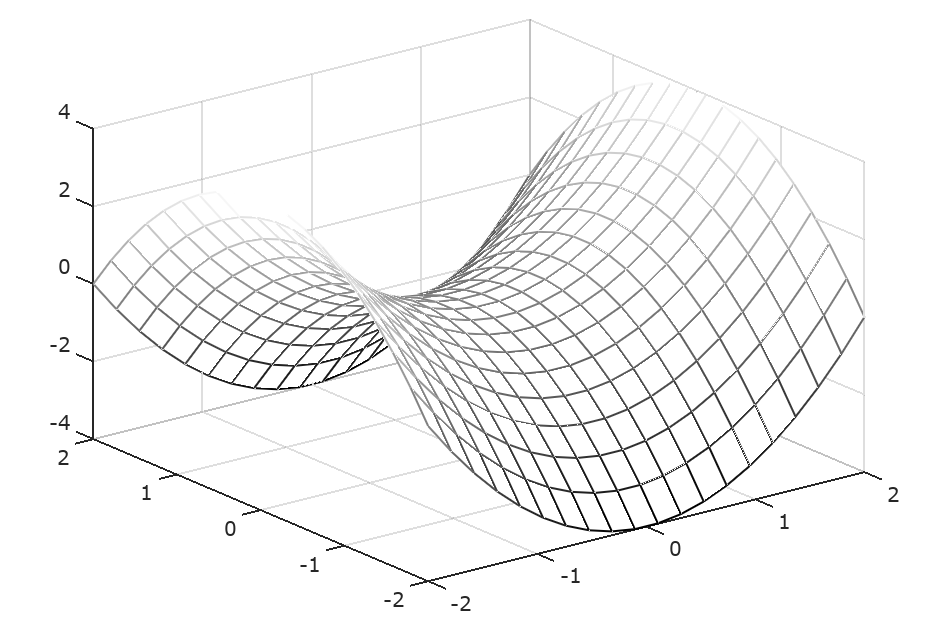
\includegraphics[scale=0.25]{./saddle-point-mono.png}}
  \caption{$f=x^2-y^2$}
  \label{x2my2}
 \end{minipage}
 \begin{minipage}{0.48\hsize}
  \centering
  \IfFileExists{2400dpi.aux}
  {\includegraphics{./convex-mono-for2400dpi.png}}
  {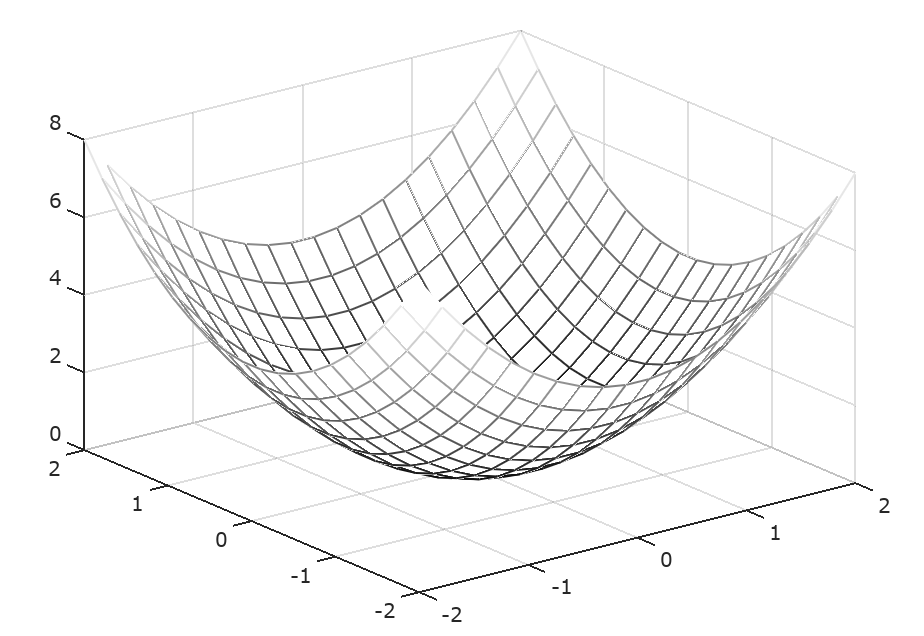
\includegraphics[scale=0.25]{./convex-mono.png}}
  \caption{$g=x^2+y^2$}
  \label{x2py2}
 \end{minipage}
\end{figure}
\vspace{0pt}

\section{エビデンス関数の最大化の式変形}
行列$\beta\trans{\Phi}\Phi$をある行列$P$で対角化する.
$$
P^{-1} \left(\beta\trans{\Phi}\Phi\right) P = \diag(\lambda_1, \ldots, \lambda_M).
$$
すると行列$A:=\alpha I + \beta\trans{\Phi}\Phi$も同じ$P$で対角化できて
$$
P^{-1} A P = \diag(\alpha + \lambda_1, \ldots, \alpha + \lambda_M).
$$
よって
$$
|A|=\prod_{i=1}^M\left(\lambda_i + \alpha\right)
$$
となる. $\alpha$で微分すると
$$
\dif{\alpha}\log |A|=\sum_{i=1}^M \frac{1}{\lambda_i + \alpha}.
$$
式(\ref{log_evidence})を$\alpha$で微分すると
$$
\dif{\alpha} \log p\left(\bm{t}\,|\,\alpha,\beta\right)=\frac{M}{2\alpha}-\half\trans{m_N}m_N - \half\sum \frac{1}{\lambda_i + \alpha}=0.
$$
よって
$$
\alpha \trans{m_N}m_N = M-\sum_{i=1}^M \frac{\alpha}{\lambda_i + \alpha}=\sum_{i=1}^M \frac{\lambda_i}{\lambda_i + \alpha}.
$$
これを$\gamma$とおくと
$$
\alpha=\frac{\gamma}{\trans{m_N}m_N}.
$$
ただし, $m_N$は陰に$\alpha$に依存しているのでこれは実は$\alpha$を含む方程式である.

$\beta$についても同様にしてみる. $\beta\trans{\Phi}\Phi$の固有値が$\lambda_i$だから$\lambda_i$は$\beta$に比例する.
つまり微分が比例係数に等しい.
$$
\dif{\beta} \lambda_i = \frac{\lambda_i}{\beta}.
$$
よって
$$
\dif{\beta} \log |A| = \sum \frac{\lambda_i/\beta}{\lambda_i + \alpha}=\frac{\gamma}{\beta}.
$$
式(\ref{log_evidence})を$\beta$で微分すると
$$
\frac{N}{2\beta} - \half\Norm{\bm{t}-\Phi m_N}^2-\frac{\gamma}{2\beta}=0.
$$
よって
$$
\frac{1}{\beta}=\frac{1}{N-\gamma}\Norm{\bm{t}-\Phi m_N}^2.
$$
\vspace{0pt}

\section{パラメータの関係}
パラメータがたくさんでてきたのでそれらの関係を見直してみよう.
まず線形基底モデルを考えた. $\phi(x)$を$M$個の基底関数からなるベクトルとする.
$x$は観測値であり,
$$
y(x,w)=\trans{w}\phi(x)
$$
とした. $\bm{t}$を観測値に対する目標値で, それは$x$によらずに精度パラメータ$\beta$に従うガウス分布とした.
$$
\fnvPair p(\bm{t}|w,\beta)=\fnvPair\calN(t|y(x,w),\beta^{-1}).
$$
ベイズ的に扱うために$w$に関して事前確率分布を与えたい. 上式が$w$に関する2次関数なので,
共役事前分布としてハイパーパラメータ$\alpha$を導入し,
$$
\fnvPair p(w|\alpha)=\fnvPair\calN(w|0, \alpha^{-1}I)
$$
を仮定した. そうすることで事後分布は
$$
\fnvPair p(w|t)=\fnvPair\calN(w|m_N,S_N)
$$
の形(ただし, $m_N=\beta S_N\trans{\Phi}t$, $S_N^{-1}=\alpha I + \beta \trans{\Phi}\Phi$)になった.

さて, ここで$\alpha$, $\beta$はハイパーパラメータではあるが, 事前分布を入れて確率変数的に扱いたい.
その上で最尤推定の手法を用いて実際のデータから値を決めるという枠組みを経験ベイズという.
そのとき$t$の予測分布は
$$
\fnvPair p(t|\bm{t})
= \int \fnvPair p(t|w,\beta)\,
       \fnvPair p(w|\bm{t},\alpha,\beta)\,
       \fnvPair p(\alpha,\beta|\bm{t})\,
       dw d\alpha d\beta
$$
となる. とはいえ, そのまま扱うのは難しいのでまずデータが十分たくさんあるとき, $\alpha$, $\beta$は殆ど固定値,
つまり$\alpha$, $\beta$の分布はある特定の値$\hat{\alpha}$, $\hat{\beta}$にデルタ関数的に近づくと仮定しよう.
$$
\fnvPair p(\alpha,\beta|\bm{t})
\approx \delta_{\alpha,\hat{\alpha}} \delta_{\beta,\hat{\beta}}.
$$
そうすると
$$
\fnvPair p(t|\bm{t})
\approx \int \fnvpair p(t|w,\hat{\beta})\,
             \fnvpair p(w|\bm{t},\hat{\alpha},\hat{\beta})\,
             dw
$$
となり予測分布は$\hat{\alpha}$, $\hat{\beta}$を求めればよいということになる.

次に$\alpha$, $\beta$を求める方法を考える. ベイズの定理から
$$
\fnvPair p(\alpha,\beta|\bm{t})
\propto \fnvPair p(\bm{t}|\alpha,\beta)\,
        p(\alpha,\beta)
$$
となる. ここで$p(\alpha,\beta)$はほぼ平坦, つまり$\alpha$, $\beta$の値はどれも同じぐらいの可能性があるという仮定を置く.
そうすると事後分布を最大化する$\alpha$, $\beta$を求める最尤推定の問題は, 尤度関数を最大化する問題に近似できる.
この尤度関数をエビデンスといい, この手法をエビデンス近似という.
そして, $\fnvPair p(\bm{t}|\alpha,\beta)$を最大化するための
$\alpha$, $\beta$の関係式を求めたのが前節であった.

以上のパラメータの関係を図\ref{para-dep}に示した.
実際には, 初期値$\alpha$, $\beta$を適当に決め, この図に従って計算して新しい$\alpha$, $\beta$を求めたあと再度繰り返す.
それが収束すればその値を採用する. ここではその収束性については議論しない.
\begin{figure}[ht]
 \begin{minipage}{1\hsize}
  \centering
  \includegraphics*[bb=0 0 260 220]{./para-dep.pdf}
  \caption{$\alpha$, $x$, $\phi$, $t$, $\beta$の関係図}
  \label{para-dep}
 \end{minipage}
\end{figure}
